\ifx\allfiles\undefined
\documentclass[12pt, a4paper, oneside, UTF8]{ctexbook}
\def\path{../config}
\usepackage{amsthm}
\usepackage{amssymb}
\usepackage{array}
\usepackage{xcolor}
\usepackage{graphicx}
\usepackage{mathrsfs}
\usepackage{enumitem}
\usepackage{geometry}
\usepackage[colorlinks, linkcolor=black]{hyperref}
\usepackage{stackengine}
\usepackage{yhmath}
\usepackage{extarrows}
\usepackage{tikz}
\usepackage{forest}
\usetikzlibrary{decorations.pathreplacing, positioning}
% \usepackage{unicode-math}
\usepackage{esint}
\usepackage{pifont}
\usepackage{tcolorbox}
\tcbuselibrary{skins, breakable}

\usepackage{multicol} 
\usepackage{fontspec} % 使用字体

\setmainfont{Times New Roman}
\setCJKmainfont{LXGWWenKai-Light}[
    SlantedFont=*
]

\usepackage{listings} % 用于插入代码

% 定义代码高亮风格
\lstset{
    basicstyle=\ttfamily\small,        % 基本字体样式(等宽小字体)
    keywordstyle=\color{blue},         % 关键字颜色
    commentstyle=\color{green},        % 注释颜色
    stringstyle=\color{red},           % 字符串颜色
    numbers=none,
    breaklines=true,                   % 自动换行
    frame=single,                      % 代码框边框
    rulecolor=\color{black},           % 边框颜色
    captionpos=b,                      % 标题位置(底部)
    showspaces=false,                  % 不显示空格标记
    showstringspaces=false,            % 不显示字符串中的空格标记
    language=C                         % 设置语言为 C
}

\usepackage{fontawesome5}

\usepackage{amsmath}
\usepackage{booktabs, array}
\usepackage{makecell}
\usepackage{fancyhdr}
\usepackage[dvipsnames, svgnames]{xcolor}
\usepackage{listings}
\usepackage{tasks}[2020/01/11]

\everymath{\displaystyle}

\definecolor{mygreen}{rgb}{0,0.6,0}
\definecolor{mygray}{rgb}{0.5,0.5,0.5}
\definecolor{mymauve}{rgb}{0.58,0,0.82}
\definecolor{NavyBlue}{RGB}{0,0,128}
\definecolor{Rhodamine}{RGB}{255,0,255}
\definecolor{PineGreen}{RGB}{0,128,0}

\graphicspath{ {figures/},{../figures/}, {config/}, {../config/} }

\linespread{1.6}

\geometry{
    top=25.4mm, 
    bottom=25.4mm, 
    left=20mm, 
    right=20mm, 
    headheight=2.17cm, 
    headsep=4mm, 
    footskip=12mm
}

\setenumerate[1]{itemsep=5pt,partopsep=0pt,parsep=\parskip,topsep=5pt}
\setitemize[1]{itemsep=5pt,partopsep=0pt,parsep=\parskip,topsep=5pt}
\setdescription{itemsep=5pt,partopsep=0pt,parsep=\parskip,topsep=5pt}



% \begin{lstlisting}[language=TeX] ... \end{lstlisting}

% 定理环境设置
% ---------- 颜色 ----------
\definecolor{ExBlue}{HTML}{4F81BD}
\definecolor{SolGreen}{HTML}{77933C}
\definecolor{DefRed}{HTML}{C5504B}
\definecolor{ThmOrange}{HTML}{E97132}
\definecolor{RemGray}{HTML}{7F7F7F}
\definecolor{CorPurple}{HTML}{7030A0}
\definecolor{ForGray}{HTML}{595959}

% ---------- 通用“变色”模板 ----------
\tcbset{
    mybox/.style n args={1}{
        enhanced, breakable,
        arc=6pt,
        boxrule=0.6pt,
        left=8pt, right=8pt, top=6pt, bottom=6pt,
        drop shadow={black!25},
        fonttitle=\bfseries,
        coltitle=white,
        colbacktitle=#1!85,
        colback=#1!10,
        colframe=#1,
    }
}

% ---------- 各环境 ----------
% 例题
\newtcolorbox{example}[1][]{mybox={ExBlue}, title={\ifstrempty{#1}{Example}{#1}}}
% 解答
\newtcolorbox{solution}[1][]{mybox={SolGreen}, title={\ifstrempty{#1}{Solution}{#1}}}
% 定义
\newtcolorbox{definition}[1][]{mybox={DefRed}, title={\ifstrempty{#1}{Definition}{#1}}}
% 定理
\newtcolorbox{theorem}[1][]{mybox={ThmOrange}, title={\ifstrempty{#1}{Theorem}{#1}}}
% 标注
\newtcolorbox{remark}[1][]{mybox={RemGray}, title={\ifstrempty{#1}{Remark}{#1}}}
% 推论
\newtcolorbox{corollary}[1][]{mybox={CorPurple}, title={\ifstrempty{#1}{Corollary}{#1}}}
% 公式
\newtcolorbox{formula}[1][]{mybox={ForGray}, title={\ifstrempty{#1}{Formula}{#1}}}


\settasks{
    label-format = \bfseries,
    label        = \Alph*.,
    label-width  = 1.2em,
    label-offset = 0.3em,
    item-indent  = 1.9em,
    column-sep   = 0.5em
}

\newenvironment{choices}[1][4]   % 默认 4 栏
    {\begin{tasks}(#1)}
    {\end{tasks}}

% 自定义命令的文件

\def\d{\mathrm{d}}
\def\R{\mathbb{R}}
\def\P{\partial} 
\newcommand{\bs}[1]{\begin{solution}#1\end{solution}}
\newcommand{\bt}[1][1]{% 默认参数为1
    \ensuremath{% 确保数学模式
        \foreach \n in {1,...,#1} {\blacktriangle}% 循环输出 #1 个黑色三角形
    }%
}

\newcommand{\bl}[1][1]{% 默认参数为1
    \ensuremath{% 确保数学模式
        \foreach \n in {1,...,#1} {\blacklozenge}% 循环输出 #1 个黑色三角形
    }%
}
\newif\ifshowanswers
%\showanswerstrue % 注释掉这行就不显示答案

% 定义答案环境
\newcommand{\answer}[1]{%
    \ifshowanswers
        #1%
    \fi
}




% 修改参数改变封面样式,0 默认原始封面、内置其他1、2、3种封面样式
\def\myIndex{3}


\ifnum\myIndex>0
    \input{\path/cover_package_\myIndex} 
\fi

\def\myTitle{冲刺150笔记}
\def\myAuthor{Weary Bird}
\def\myDateCover{\today}
\def\myDateForeword{\today}
\def\myForeword{行香子}
\def\myForewordText{
树绕村庄,水满陂塘;倚东风、豪兴徜徉。小园几许,收尽春光。有桃花红,李花白,菜花黄。 \\
远远苔墙,隐隐茅堂;飏青旗、流水桥旁。偶然乘兴,步过东冈。正莺儿啼,燕儿舞,蝶儿忙。 \\
}
\def\mySubheading{知错能改善莫大焉}


\begin{document}
% \input{../config/cover}
\else
\fi
\chapter{数据结构}
\section{选择题}
\begin{enumerate}
    \item \bt 下列程序段的时间复杂度是\_\_\_\_ 
    \begin{lstlisting}[language=C]
int sum = 0;
    for(int i = 1; i < n; i *= 2)
        for(int j = 0; j < i; j++)
            sum++;
    \end{lstlisting}

    \item 若长度为n的非空线性表采用顺序存储结构,在表的第$i$个位置插入一个数据元素,则$i$的合法位置
    应该是(   )
    \begin{choices}
        \task $1\leq i \leq n$ 
        \task $1\leq i \leq n + 1$
        \task $0\leq i \leq n - 1$
        \task $0\leq i \leq n$
    \end{choices}

    \item 关于线性表的顺序存储和链式存储结构的描述中,正确的是(    ) 
    \begin{enumerate}
        \item [(1)] 线性表的顺序结构优于其链式存储结构
        \item [(2)] 链式存储结构比顺序存储结构能更方便地表示各种逻辑结构
        \item [(3)] 若频繁使用插入和删除操作,则顺序存储结构更优于链式存储结构
        \item [(4)] 顺序存储结构和链式存储结构都可以进行顺序存取 
    \end{enumerate}
    \begin{choices}
        \task 1,2,3
        \task 2,4
        \task 2,3
        \task 3,4
    \end{choices}

    \item 对于一个头指针位$head$的带头结点的单链表,判断该表为空表的条件是(   ),对于不带头结点
    的单链表,判断空表的条件是(   ) 
    \begin{choices}[2]
        \task $head == NULL$ 
        \task $head\rightarrow next == NULL$ 
        \task $head\rightarrow next == head$ 
        \task $head \neq NULL$
    \end{choices}

    \item 一个链表最常用的操作为在末尾插入结点和删除节点,则选用(   )最节省时间. 
    \begin{choices}[2]
        \task 带头结点的双循环链表
        \task 单循环列表
        \task 带尾结点的单循环链表
        \task 单链表
    \end{choices}

    \item 设对$n(n>1)$元素的线性表运算只有4种,删除第一个元素,删除最后一个元素,在第一个元素之前插入
    一个元素,在最后一个元素之后插入一个元素,则最好使用(    ) 
    \begin{choices}[1]
        \task 只有尾结点指针没有头结点指针的循环单链表
        \task 只有尾结点指针没有头结点指针的非循环双链表
        \task 只有头结点指针没有尾结点指针的循环双链表
        \task 既有头结点有又有尾结点的循环单链表
    \end{choices}

    \item 数的路径长度是从树根到每个结点的路径长度的(   ) 
    \begin{choices}
        \task 总和
        \task 最小值
        \task 最大值
        \task 平均值
    \end{choices}

    \item (判断正误) 
    \begin{enumerate}
        \item [(1)] 度为2的有序树就是二叉树
        \item [(2)] 结点按完全二叉树层序编号的二叉树中,第$i$个结点的左孩子编号为$2i$ 
    \end{enumerate}

    \item 具有10个叶结点的二叉树中有(   )个度为2的结点 
    
    \item 设二叉树有$2n$个结点,且$m<n$,则不可能存在(   )的结点 
    \begin{choices}
        \task n个度为0
        \task 2m个度为0
        \task 2m个度为1
        \task 2m个度为2
    \end{choices}

    \item 一颗完全二叉树上有1001个结点,其中叶结点的个数是(    ) 

    \item \bl 对于任意一颗高度为5且有10个结点的二叉树,若采用顺序存储结构保存,每个节点占1个存储单元(仅保存
    结点的数据信息),则存放该二叉树需要的存储单元数量至少是(     ) 

    \item 在下列关于二叉树遍历的说法中,正确的是(     ) 
    \begin{choices}[1]
    \task 若有一个结点是二叉树中某个子树的中序遍历结果序列的最后一个结点,则它一定是该子树的前序遍历结果序列的最后一个结点。
    \task 若有一个结点是二叉树中某个子树的前序遍历结果序列的最后一个结点,则它一定是该子树的中序遍历结果序列的最后一个结点。
    \task 若有一个叶结点是二叉树中某个子树的中序遍历结果序列的最后一个结点,则它一定是该子树的前序遍历结果序列的最后一个结点。
    \task 若有一个叶结点是二叉树中某个子树的前序遍历结果序列的最后一个结点,则它一定是该子树的中序遍历结果序列的最后一个结点。
    \end{choices} 

    \item 设$n,m$为一颗二叉树上的两个结点,在后序遍历时,$n$在$m$前的充分条件是(    ) 
    \begin{choices}
        \task n在m的右方 
        \task n是m的祖先
        \task n在m的左方
        \task n是m的子孙 
    \end{choices}

    \item 在二叉树中的两个结点m和n,若m是n的祖先,则使用(    )可以找到从m到n的路径 
    
    \item 若二叉树中结点的先序序列是$\ldots a\ldots b\ldots$,中序序列是$\ldots b\ldots a\ldots$则(    ) 
    \begin{choices}[1]
        \task 结点a和结点b分别在某结点的左子树和右子树中
        \task 结点b和结点a的右孩子中
        \task 结点b在结点a的左孩子中
        \task 结点a和结点b分别在某结点的两颗分非空子树中 
    \end{choices}

    \item 线索二叉树是(    )结构 
    \begin{choices}
        \task 逻辑
        \task 逻辑和存储
        \task 物理
        \task 线性
    \end{choices}

    \item 一颗左子树为空的二叉树的先序线索化后,其中空的链域的个数是(    ) 
    \begin{choices}
        \task 不确定
        \task 0个
        \task 1个
        \task 2个
    \end{choices} 

    \item 二叉树在线索化后,仍然不能有效求解的问题是(    ) 
    \begin{choices}[2]
        \task 先序线索二叉树求先序后继
        \task 中序线索二叉树求中序后继
        \task 中序线索二叉树求中序前驱
        \task 后序线索二叉树求后序后继 
    \end{choices}

    \item 若X是二叉中序线索树中一个有左孩子的结点,且X不为根,则X的前缀为(    ) 
    \begin{choices}[2]
        \task X的双亲
        \task X的右子树中最左节点
        \task X的左子树中最右结点
        \task X的左子树中最右的叶结点
    \end{choices}

    \item (   )遍历仍然需要栈的支持. 
    \begin{choices}
        \task 先序线索树
        \task 中序线索树
        \task 后序线索树 
        \task 所有线索树 
    \end{choices}

    \item \bl 先序序列为\underline{a,b,c,d}的不同二叉树的个数是(      ) 

    \item \bl 若结点p和q在二叉树T的中序遍历序列中相邻,且p在q之前,则下列p和q的关系中,不可能的是(    )
    \begin{enumerate}
        \item [(1)] q是p的双亲 
        \item [(2)] q是p的右孩子
        \item [(3)] q是p的右兄弟
        \item [(4)] q是p的双亲的双亲
    \end{enumerate}
    \begin{choices}
        \task 1 
        \task 3
        \task 2,3
        \task 2,4
    \end{choices}

    \item 利用二叉链表存储森林时,根结点的右指针是(    ) 
    \begin{choices}
        \task 指向最左兄弟 
        \task 指向最右兄弟 
        \task 一定为空
        \task 不一定为空 
    \end{choices}

    \item 森林$T=(T_1,T_2,\ldots,T_m)$转换为二叉树BT的过程为:若m=0,则BT为空,若$m\neq 0$,则(    ) 
    \begin{choices}[1]
        \task 将中间子树$T_{mid}(mid=(1+m)/2)$的根作为BT的根;将$(T_1,T_2,\ldots,T_{mid-1})$转换为BT的左子树;
        将$(T_{mid+1},\ldots,T_m)$转换为BT的右子树 
        \task 将子树$T_1$的根作为BT的根,将$T_1$的子树森林转换为BT的左子树;将$(T_2,T_3\ldots,T_m)$转换BT的右子树 
        \task 将子树$T_1$根作为BT的根,将$T_1$的左子森林转换为BT的左子树;右子森林转换右子树,其他类似 
        \task 将森林T的根作为BT的根,将$(T_1,\ldots,T_m)$转换为该根下的结点,得到一棵树,然后将这课树转换为二叉树 
    \end{choices}

    \item 设F是一个森林,B是由F转换为来的二叉树.若F中有n个非终端节点,则B中右指针域为空的结点数目是(    ) 

    \item \bl 将森林转换为对应的二叉树,若二叉树中,结点u是结点v的父结点的父结点,则原来的森林中,u和v可能具有关系是(   ) 
    \begin{enumerate}
        \item [(1)] 父子关系 
        \item [(2)] 兄弟关系
        \item [(3)] u的父结点和v的父结点是兄弟关系
    \end{enumerate}
    \begin{choices}
        \task 2 
        \task 1,2
        \task 1,3
        \task 1,2,3 
    \end{choices}

    \item \bl 已知一颗有2011个结点的树,其叶结点个数为116,则该树对应的二叉树中无右孩子的结点个数为(   )
    \begin{choices}
        \task 115
        \task 116
        \task 1895
        \task 1896
    \end{choices}

    \item \bl 若森林F有15条边,25个结点,则F包含树的个数是(    ) 

    \item \bl 若将一颗树T转换为对应的二叉树BT,则下列对BT的遍历中,其遍历序列与T的后根遍历序列相同的是(   ) 
    \begin{choices}
        \task 先序遍历
        \task 中序遍历
        \task 后序遍历
        \task 层序遍历
    \end{choices}

    \item 在有n个叶节点的哈夫曼树中,非叶结点的总数是(   ) 
    
    \item 设哈夫曼编码的长度不超过4,若已对两个字符编码为1和01,则还最多可以对(   )个个字符编码 
    
    \item 一下对于哈夫曼树的说法中,错误的是(    ) 
    \begin{choices}[1]
        \task 对应一组权值构造出来的哈夫曼树一般不是唯一的
        \task 哈夫曼树具有最小的带权路径长度
        \task 哈夫曼树中没有度为1的结点
        \task 哈夫曼树中除了度为1的节点外,还有度为2的结点和叶结点 
    \end{choices}

    \item 若度为m的哈夫曼树中,叶结点的数目为n,则非叶结点的数目为(     ) 
    
    \item \bl 已知字符集\underline{a,b,c,d,e,f}若各字符出现的次数分别为\underline{6,3,8,2,10,4}则对应字符集中的
    各字符的哈夫曼编码可能是(    ) 
    \begin{choices}[2]
        \task \underline{00,1011,01,1010,11,100} 
        \task \underline{00,100,110,000,0010,01}
        \task \underline{10,1011,11,0011,00,010}
        \task \underline{0011,10,11,0010,01,000}
    \end{choices}

    \item \bl 对应任意给定的含有n个字符的有限集合S,用二叉树表示S的哈夫曼编码集和定长编码集,分别得到二叉树$T_1$和$T_2$.下列叙述
    正确的是(    ) 
    \begin{choices}[1]
        \task $T_1$和$T_2$的结点数相同
        \task $T_1$的高度大于$T_2$的高度
        \task 出现频次不同的字符在$T_1$中处于不同的层
        \task 出现频次不同的字符在$T_2$中处于相同的层
    \end{choices}

    \item 带权有向图G用临接矩阵存储,则$v_i$的入度等于邻接矩阵中(    )
    \begin{choices}[2]
        \task 第i行非$\infty$的元素个数
        \task 第i列非$\infty$的元素个数
        \task 第i行非$\infty$且非0的元素个数
        \task 第i列非$\infty$且非0的元素个数
    \end{choices}

    \item n个顶点的无向图的邻接表中最多有(   )个边表节点
    
    \item 假设有n个顶点,e条边的有向图用邻接表表示,则删除与某个顶点v相关的所有边的
    时间复杂度是(    ) 

    \item 对于一个有n个顶点,e条边的图采用临接表表示时,进行DFS遍历的时间复杂度是(   ),空间复杂度是
    (   );进行BFS遍历的时间复杂度是(   ),空间复杂度是(    ) 

    \item 对于一个有n个顶点,e条边的图采用临接矩阵表示时,进行DFS遍历的时间复杂度是(   ),空间复杂度是
    (   );进行BFS遍历的时间复杂度是(   ),空间复杂度是(    ) 

    \item 图的广度优先生成树的树高比深度优先生成的树高(    ) 
    \begin{choices}
        \task 小或相等
        \task 小 
        \task 大或相等 
        \task 大
    \end{choices}

    \item 一下叙述中,正确的是(   ) 
    \begin{choices}[1]
        \task 最短路径一定是简单路径
        \task Dijkstra算法不适合求有环路的带权图的最短路径
        \task Dijkstra算法不适合求任意两个顶点的最短路径 
        \task Floyd算法求两个顶点的最短路径,$path_k-1$一定是$path_k$的子集 
    \end{choices}

    \item 若一个有向图的顶点不能排成一个拓扑序列,则可以判断该有向图(    ) 
    \begin{choices}[2]
        \task 含有多个出度为0的顶点
        \task 是一个强连通图
        \task 含有多个入度为0的顶点
        \task 含有顶点数大于1的强连通分量 
    \end{choices}

    \item 下列关于图的说法中,正确的是(   ) 
    \begin{enumerate}
        \item [(1)] 有向图中顶点V的度等于其临接矩阵中第V行中1的个数
        \item [(2)] 无向图的邻接矩阵一定是对称矩阵,有向图的邻接矩阵一定是非对称矩阵
        \item [(3)] 在带权图$G$的最小生成树$G_i$中,某条边的权值可能会超过为选边的权值
        \item [(4)] 若有向无环图的拓扑序列唯一,则可以唯一确定该图 
    \end{enumerate}
    \begin{choices}
        \task 1,2,3
        \task 3,4
        \task 3
        \task 4
    \end{choices}

    \item 已知带权图为$G=(V,E)$,其中$V=\{v_1,v_2,\ldots,v_{10}\}$,边集合为$E=\{<v_1,v_2>5,
    <v_1,v_3>6,<v_2,v_5>3,<v_3,v_5>6,<v_3,v_4>3,<v_4,v_5>3,<v_4,v_7>1,<v_4,v_8>4,<v_5,v_6>4,
    <v_5,v_7>2,<v_6,v_{10}>4,<v_7,v_9>5,<v_8,v_9>2,<v_9,v_{10}>2\}$则G的关键路径长度为(   ) 

    \answer{
        
    }

    \item 下列关于关键路径的说法中,正确的是(   ) 
    \begin{enumerate}
        \item [(1)]改变网上某一关键路径上的某一关键路径,必将产生不同的关键路径
        \item [(2)]在AOE图中,关键路径上活动的时间延长多少,整个工期的时间也就随之延长多少
        \item [(3)]缩短关键路径上任意一个关键活动的持续时间可缩短关键路径长度
        \item [(4)]缩短所有关键路径上共有的任意一个关键活动的持续时间可缩短关键路径的长度
        \item [(5)]缩短多条关键路径上共有的任意一个关键活动的持续时间可缩短关键路径长度 
    \end{enumerate}
    \begin{choices}
        \task 2,5
        \task 1,2,4
        \task 2,4
        \task 1,4
    \end{choices}

    \item \bl 若用临接矩阵存储有向图,矩阵中主对角线以下的元素全为零,则关于该图拓扑序列的结论是(   )
    \begin{choices}[2]
        \task 存在,且唯一
        \task 存在,且不唯一
        \task 存在,可能唯一
        \task 无法确定是否存在
    \end{choices}

    \item \bl 对下列图所示的有向带权图,若采用Dijkstra算法求源点a到其他个顶点的最短路径,则得到的
    的第一条最短路径的目标顶点是b,第二条最短路径的目标顶点是c,后续得到的其余各最短路径的目标顶点一次是(   )
    \begin{center}
        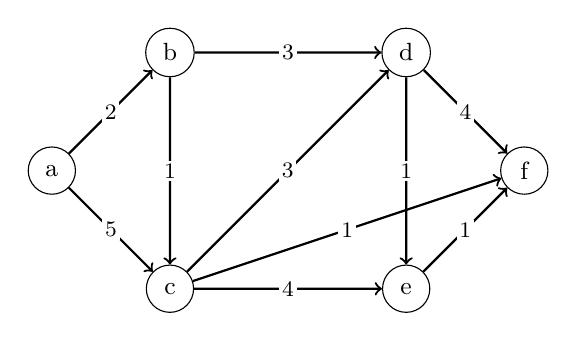
\begin{tikzpicture}[scale=1.5,
        vertex/.style={circle, draw, minimum size=6mm, font=\small},
        edge/.style={->, thick},
        label/.style={font=\footnotesize, pos=.5, auto=center, fill=white, inner sep=1pt}
    ]

    % 顶点
    \node[vertex] (a) at (-2,-2) {a};
    \node[vertex] (b) at (-1,-1) {b};
    \node[vertex] (c) at (-1,-3) {c};
    \node[vertex] (d) at (1,-1) {d};
    \node[vertex] (e) at (1,-3) {e};
    \node[vertex] (f) at (2,-2) {f};

    % 有向边
    \draw[edge] (a) -- node[label] {2} (b);
    \draw[edge] (a) -- node[label] {5} (c);
    \draw[edge] (b) -- node[label] {1} (c);
    \draw[edge] (b) -- node[label] {3} (d);
    \draw[edge] (c) -- node[label] {3} (d);
    \draw[edge] (c) -- node[label] {1} (f);
    \draw[edge] (c) -- node[label] {4} (e);
    \draw[edge] (d) -- node[label] {1} (e);
    \draw[edge] (d) -- node[label] {4} (f);
    \draw[edge] (e) -- node[label] {1} (f);

    \end{tikzpicture}
    \end{center}
    \begin{choices}
        \task d,e,f 
        \task e,d,f 
        \task f,d,e 
        \task f,e,d
    \end{choices}


    \item \bl 使用Dijkstra算法求下图中从顶点1到其他个顶点的最短路径,依次得到的各最短路径的目标
    顶点是(   )

    \begin{center}
    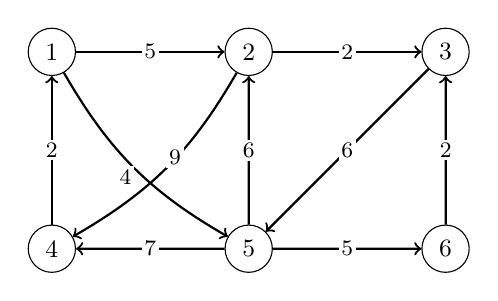
\begin{tikzpicture}[scale=2.5,
    vertex/.style={circle, draw, minimum size=6mm, font=\small},
    edge/.style={->, thick},
    label/.style={font=\footnotesize, pos=.5, auto=center, fill=white, inner sep=1pt}
    ]

    % 顶点
    \node[vertex] (1) at (0,0) {1};
    \node[vertex] (2) at (1,0) {2};
    \node[vertex] (3) at (2,0) {3};
    \node[vertex] (4) at (0,-1) {4};
    \node[vertex] (5) at (1,-1) {5};
    \node[vertex] (6) at (2,-1) {6};

    % 有向边(1→5 用弧线下弯,2→4 用弧线上弯)
    \draw[edge,bend right=15] (1) to node[label,below left=-1pt] {4} (5);
    \draw[edge,bend left =15] (2) to node[label,above right=-1pt] {9} (4);

    % 其余直线边
    \draw[edge] (1) -- node[label] {5} (2);
    \draw[edge] (2) -- node[label] {2} (3);
    \draw[edge] (3) -- node[label] {6} (5);
    \draw[edge] (4) -- node[label] {2} (1);
    \draw[edge] (5) -- node[label] {6} (2);
    \draw[edge] (5) -- node[label] {7} (4);
    \draw[edge] (5) -- node[label] {5} (6);
    \draw[edge] (6) -- node[label] {2} (3);

    \end{tikzpicture}
    \end{center}

    \begin{choices}
        \task 5,2,3,4,6
        \task 5,2,3,6,4
        \task 5,2,4,3,6
        \task 5,2,6,3,4
    \end{choices}

    \item \bl 下列所示的AOE网表示一项包含8个活动的工程,活动d的最早开始时间和最迟开始时间分别是(   ) 

    \begin{center}
    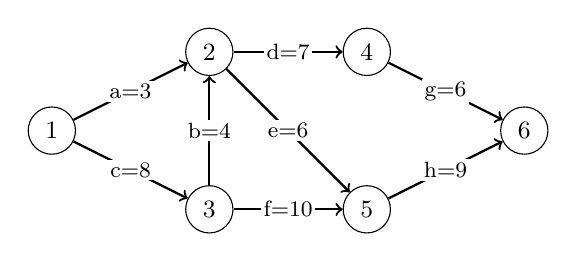
\begin{tikzpicture}[scale=2,
    vertex/.style={circle, draw, minimum size=6mm, font=\small},
    edge/.style={->, thick},
    label/.style={font=\footnotesize, pos=.5, auto=center, fill=white, inner sep=1pt}
    ]

    % 顶点
    \node[vertex] (1) at (0,0) {1};
    \node[vertex] (2) at (1,0.5) {2};
    \node[vertex] (3) at (1,-0.5) {3};
    \node[vertex] (4) at (2,0.5) {4};
    \node[vertex] (5) at (2,-0.5) {5};
    \node[vertex] (6) at (3,0) {6};

    \draw[edge] (1) -- node[label] {a=3} (2);
    \draw[edge] (1) -- node[label] {c=8} (3);
    \draw[edge] (2) -- node[label] {d=7} (4);
    \draw[edge] (2) -- node[label] {e=6} (5);
    \draw[edge] (3) -- node[label] {b=4} (2);
    \draw[edge] (3) -- node[label] {f=10} (5);
    \draw[edge] (4) -- node[label] {g=6} (6);
    \draw[edge] (5) -- node[label] {h=9} (6);
    \end{tikzpicture}
    \end{center}
    \begin{choices}
        \task 3,7
        \task 12,12
        \task 12,14
        \task 15,15
    \end{choices}

    \item 由n个数据元素组成的两个表:一个递增有序,一个无序.采用顺序查找算法,对有序表从头开始查找,发现当前
    元素已不小于待查元素时,停止查找,确定查找不成功,已知查找任意元素的概率是相同的,则在两种表中成功查找(   ) 
    \begin{choices}[2]
        \task 平均时间后者小
        \task 平均时间两者相同
        \task 平均时间前者小
        \task 无法确定
    \end{choices}

    \item 在一个顺序存储的有序线性表上查找一个数据时,既可以采用折半查找,也可以采用顺序查找,但前者
    比后者的查找速度(   ) 
    \begin{choices}[2]
        \task 必然快
        \task 取决于表是递增还是递减
        \task 在大部分情况下要快
        \task 必然不快 
    \end{choices}

    \item 折半查找过程所对应的判断树是一颗(   ) 
    \begin{choices}
        \task 最小生成树
        \task 平衡二叉树
        \task 完全二叉树
        \task 满二叉树
    \end{choices}

    \item 折半查找和二叉排序树的时间性能(   ) 
    \begin{choices}
        \task 相同
        \task 有时不相同
        \task 完全不同
        \task 无法比较
    \end{choices}

    \item 对表长为n的有序表进行折半查找,其判定树的高度为(    ) 
    \begin{choices}
        \task $\lceil\log_{2}{(n+1)}\rceil$
        \task $\log_{2}{(n+1)}-1$
        \task $\lceil\log_{2}{n}\rceil$
        \task $\lfloor\log_2{n}\rfloor$ - 1
    \end{choices}

    \item 具有12个关键字的有序表中,对每个关键的查找概率相同,折半查找算法查找成功的平均查找长度是(   ),
    折半查找失败的平均查找长度是(    ) 

    \item 为提高查找效率,对有65025个元素的有序顺序表建立索引顺序结构,在最好的情况下查找到表中亦有元素最多
    需要执行(   )次关键字比较 

    \item \bl 已知一个长度为16的顺序表L,其元素按关键字有序排列,若采用折半查找法查找一个L中不存在的元素,则
    关键字的比较次数最多是(    ) 

    \item 在含有n个结点的二叉排序中查找某个关键字的结点时,最多进行(   )比较 
    \item 构建一颗具有n个节点的二叉排序树时,最理想情况下的深度为(   )
    \item 含有20个节点的平衡二叉树的最大深度为(   )
    \item 具有5层结点的AVL树至少有(   )个结点

    \item 下列关于红黑树的说法中,正确的是(   ) 
    \begin{choices}[1]
        \task 红黑树的红结点的数目最多和黑结点的数目相同
        \task 若红黑树的所有结点都是黑色的,那么它一定是一棵满二叉树
        \task 红黑树的任何一个分支结点都有两个非空孩子结点
        \task 红黑树的子树也一定是红黑树
    \end{choices}

    \item \bt 将关键字序列\underline{1,2,3,4,5,6,7}一次插入初始为空的红黑树T,则T中红结点的个数是(    ) 
    \item \bl 现有一颗无重复关键字的平衡二叉树,对其进行中序遍历得到一个降序序列,下列关于该平衡二叉树的叙述中,正确的是(  ) 
    \begin{choices}[2]
        \task 根结点的度一定是2
        \task 树中最小元素一定是叶结点
        \task 最后插入的元素一定是叶结点
        \task 树中最大元素一定是无左子树
    \end{choices}

    \item \bl 在任意一颗非空平衡二叉树$T_1$中,删除某结点v之后形成平衡二叉树$T_2$,再将v插入$T_2$形成
    平衡二叉树$T_3$下列关于$T_1,T_3$的描述中,正确的是(   )
    \begin{enumerate}
        \item [(1)] 若v是$T_1$的叶结点,则$T_1$和$T_3$可能不相同 
        \item [(2)] 若v不是$T_1$的叶结点,则$T_1$和$T_3$一定不相同
        \item [(3)] 若v不是$T_1$的叶节点,则$T_1$和$T_3$一定相同 
    \end{enumerate}
    \begin{choices}
        \task 1
        \task 2
        \task 1,2
        \task 1,3
    \end{choices}
    \item 下列关于B与B+树的描述中,不正确的是(   ) 
    \begin{choices}[2]
        \task B数和B+树都能有效的支持顺序查找
        \task B树和B+树都能有效的支持随机查找
        \task B树和B+树都是平衡的二叉树
        \task B树和B+树都可以用于文件索引结构
    \end{choices}

    \item \bl 已知一颗3阶B树,如下图所示.删除关键字78得到一颗新B树,其最右叶结点中的关键字是(   )
    \begin{center}
        \begin{forest}
        for tree={
        rectangle,           % 方框
        draw,                % 画边
        minimum size=6mm,    % 宽、高最小 6 mm
        inner sep=2pt,       % 文字与框距离
        edge=-               % 去掉箭头(默认是无箭头实线)
        }
    [45
        [
            17 35 
            [10][21][37]
        ]
        [
            55 65
            [47][60 62][78]
        ]
    ]
        \end{forest}
    \end{center}

    \item \bl 在一颗高度为2的5阶B树中,所含有的关键的个数至少是(   ) 
    \begin{choices}
        \task 5
        \task 7
        \task 8
        \task 14
    \end{choices}

    \item \bl 下列应用中,适合使用B+树的是(   ) 
    \begin{choices}[2]
        \task 编译器中的词法分析
        \task 关系数据库系统的索引
        \task 网络中的路由表的快速查找
        \task 操作系统的磁盘空闲块管理
    \end{choices}

    \item 在开放定址法中散列到同一地址而引起的堆积问题是由于(   )而引起的
    \begin{choices}[2]
        \task 同义词之间发生冲突
        \task 非同义词之间发生冲突
        \task 同义词之间或非同义词之间发生冲突 
        \task 散列表溢出 
    \end{choices}

    \item 下列关于散列冲突处理方法中,正确的是(   ) 
    \begin{enumerate}
        \item [(1)] 采用在平方探测法处理冲突时不容易产生聚集
        \item [(2)] 采用线性探测法解决冲突时,所有同义词在散列表中一定相邻
        \item [(3)] 采用链地址法处理冲突时,若限定在链首插入,则插入任意一个元素的时间是相同的 
        \item [(4)] 采用链地址法处理冲突时容易引起聚集现象
    \end{enumerate}

    \item 对包含n个元素的散列表进行查找,平均查找长度为(   ) 
    \begin{choices}
        \task 为$O(\log_{2}{n})$
        \task 为$O(1)$
        \task 不直接依赖于n
        \task 直接依赖于表长m
    \end{choices}

    \item \bl 现有长度为11且初始为空的散列表HT,散列函数$H(k)=k\%7$,用线性探测再散列法法解决冲突,将
    关键字序列\underline{87,40,30,6,11,22,98,20}依次插入HT后,HT查找失败的平均查找长度是(   )
    \begin{choices}
        \task 4
        \task 5.25
        \task 6
        \task 6.29
    \end{choices}

    \item \bl 下列因素中,影响哈希方法的平均查找长度是(   ) 
    \begin{enumerate}
        \item [(1)] 装填因子
        \item [(2)] 散列函数
        \item [(3)] 冲突解决策略
    \end{enumerate}
    \begin{choices}
        \task 1,2
        \task 1,3
        \task 2,3
        \task 1,2,3
    \end{choices}

    \item 下列关于排序的叙述中,正确的是(   ) 
    \begin{choices}[1]
        \task 稳定的排序方法优于不稳定的排序方法
        \task 对同一线性表使用不同的排序方法进行排序,得到的排序结果可能不同
        \task 排序方法都是在顺序表上实现的,在链表上无法实现排序方法
        \task 在顺序表上实现的排序方法在链表上也可以实现
    \end{choices}

    \item 对于任意7个关键字进行基于比较的排序,至少要进行()次关键字之间的比较
    \begin{choices}
        \task 13
        \task 14
        \task 15
        \task 16
    \end{choices}

    \item 用直接插入排序算法对下列4个表进行排序(从小到大),比较次数最少的是(   ) 
    \begin{choices}[2]
        \task \underline{94,32,40,90,80,46,21,69}
        \task \underline{21,32,46,40,80,69,90,94}
        \task \underline{32,40,21,46,69,94,90,80}
        \task \underline{90,69,80,46,21,32,94,40}
    \end{choices}

    \item 对序列\underline{98,36,9,0,47,23,1,8,10,7}采用希尔排序,下列序列( )是增量为4的一趟排序结果 
    \begin{choices}[2]
        \task \underline{10,7,-9,0,47,23,1,8,98,36}
        \task \underline{-9,0,36,98,1,8,23,47,7,10}
        \task \underline{36,98,-9,0,23,47,1,8,7,10}
        \task 以上都不对
    \end{choices}

    \item 若用冒泡排序算法对序列\underline{10,14,26,29,41,52}从大到小进行排序,则需要进行(  )比较 
    \begin{choices}
        \task 3
        \task 10
        \task 15
        \task 25
    \end{choices}

    \item 一组记录的关键码为\underline{46,79,56,38,40,84},采用快速排序,以第一个记录为基准,从小到大得到
    的一次划分结果为(   ) 
    \begin{choices}[2]
        \task \underline{38,40,46,56,79,84}
        \task \underline{40,38,46,79,56,84}
        \task \underline{40,38,46,56,79,84}
        \task \underline{40,38,46,84,56,79}
    \end{choices}

    \item 快速排序算法在()情况下不利于其发挥长处 
    \begin{choices}[2]
        \task 要排序的数据量太大
        \task 要排序的数据中包含多个相同的值
        \task 要排序的数据个数为奇数
        \task 要排序的数据基本有序
    \end{choices}

    \item 对下列关键字序列用到了快排进行排序,速度最快的情形是()速度最慢的是() 
    \begin{choices}[2]
        \task \underline{21,25,5,17,9,23,30}
        \task \underline{25,23,30,17,21,5,9}
        \task \underline{21,9,17,30,25,23,5}
        \task \underline{5,9,17,21,23,25,30}
    \end{choices}

    \item 对于下列4个序列,以第一个关键字为基准用快速排序算法进行排序,在第一趟过程中移动记录次数最多的是()
    \begin{choices}[2]
        \task \underline{92,96,88,42,30,35,110,100}
        \task \underline{92,96,100,110,42,35,30,88}
        \task \underline{100,96,92,35,30,110,88,42}
        \task \underline{42,30,35,92,100,96,88,110}
    \end{choices}


    \item 设线性表中每个元素有两个数据项$k_1,k_2$现对线性表按以下规则进行排序,先看数据项$k_1$,若比其值
    小的元素在前,大的元素在后,与其值相同再看$k_2$,小的元素在前,大的元素在后.满足这种要求的算法是(   ) 
    \begin{choices}[1]
        \task 先按$k_1$进行直接插入排序,在按$k_2$进行简单选择排序
        \task 先按$k_2$进行直接插入排序,在按$k_1$进行简单选择排序
        \task 先按$k_1$进行简单选择排序,在按$k_2$进行直接插入排序
        \task 先按$k_2$进行简单选择排序,在按$k_1$进行直接插入排序
    \end{choices}

    \item 若只想得到1000个元素组成的序列中第10个最小元素之前的部分排序的序列,则用()方法最快. 
    \begin{choices}
        \task 冒泡排序
        \task 快速排序
        \task 希尔排序
        \task 堆排序
    \end{choices}

    \item 在含有n个关键字的小根堆中,关键字最大的记录可能存储在(   )位置 
    \begin{choices}
        \task n/2 
        \task n/2 + 2 
        \task 1
        \task n/2 - 1
    \end{choices}

    \item 构建n个记录的初始堆,其时间复杂度为(),对n个记录进行堆排序,最坏情况下时间复杂度是()
    \begin{choices}
        \task $O(n)$
        \task $o(n^2)$
        \task $O(\log_2{n})$
        \task $O(n\log_2{n})$
    \end{choices}

    \item 对关键字\underline{23,17,72,60,25,8,68,71,52}进行堆排序,输出两个最小关键码后的剩余堆堆是()
    \begin{choices}[2]
        \task \underline{23,72,60,25,68,71,52}
        \task \underline{23,25,52,60,71,72,68}
        \task \underline{71,25,23,52,60,72,68}
        \task \underline{23,25,68,52,60,72,71}
    \end{choices}

    \item 已知小根堆为\underline{8,15,10,21,34,16,12}删除关键字8之后需要重新建堆,关键字之间的比较次数是()
    \begin{choices}
        \task 1
        \task 2
        \task 3
        \task 4
    \end{choices}

    \item 将序列\underline{6,1,5,9,8,4,7}建成大根堆时,正确的序列变化时() 
    \begin{choices}[1]
        \task 6,1,7,9,8,4,5$\rightarrow$6,9,7,1,8,4,5$\rightarrow$9,6,7,1,8,4,5$\rightarrow$9,8,7,1,6,4,5
        \task 6,9,5,1,8,4,7$\rightarrow$6,9,7,1,8,4,5$\rightarrow$9,6,7,1,8,4,5$\rightarrow$9,8,7,1,6,4,5
        \task 6,9,5,1,8,4,7$\rightarrow$9,6,5,1,8,4,7$\rightarrow$9,6,7,1,8,4,5$\rightarrow$9,8,7,1,6,4,5
        \task 6,1,7,9,8,4,5$\rightarrow$7,1,6,9,8,4,5$\rightarrow$7,9,6,1,8,4,5$\rightarrow$9,7,6,1,8,4,5$\rightarrow$9,8,6,1,7,4,5
    \end{choices}

    \item 下列关于大根堆(至少包含两个元素)的叙述中,正确的是()
    \begin{enumerate}
        \item [(1)]可以将堆视为一颗完全二叉树
        \item [(2)]可以采用顺序存储方式保存堆
        \item [(3)]可以将堆视为一棵二叉排序树
        \item [(4)]堆中的次大值一定在根的下一层
    \end{enumerate}
    \begin{choices}
        \task 1,2
        \task 2,3
        \task 1,2,4
        \task 1,3,4
    \end{choices}

    \item 若对27个元素值进行三趟多路归并排序,则选取的归并路数最少是() 
    \begin{choices}
        \task 2
        \task 3
        \task 4
        \task 5
    \end{choices}

    \item 将两个各有N个元素的有序表合并为一个有序表,最少的比较次数(),最多比较次数是() 
    \begin{choices}
        \task N 
        \task 2N-1 
        \task 2N 
        \task N-1 
    \end{choices}

    \item 若要求排序是稳定的,且关键字为实数,则在下列排序中应该选用() 
    \begin{choices}
        \task 直接插入排序
        \task 选择排序
        \task 基数排序
        \task 快速排序 
    \end{choices}

    \item 下列排序算法中属于稳定排序的是(),平均时间复杂度为$O(n\log{n})$的是(),在最好的情况下,
    时间复杂度可以达到线性的时间有() 
    \begin{choices}[4]
        \task 冒泡排序
        \task 堆排序
        \task 选择排序 
        \task 直接插入排序 
        \task 希尔排序 
        \task 归并排序 
        \task 快速排序
    \end{choices}

    \item 若序列的原始状态为\underline{1,2,3,4,5,10,6,7,8,9}要想使得排序过程中元素比较次数最少,则应该采用的是()
    \begin{choices}
        \task 插入排序 
        \task 选择排序 
        \task 希尔排序 
        \task 冒泡排序 
    \end{choices}

    \item \bl 下列排序方法中,若将顺序存储转换为链式存储,则算法时间效率会降低的是() 
    \begin{choices}[3]
        \task 插入排序 
        \task 选择排序
        \task 冒泡排序
        \task 希尔排序 
        \task 堆排序 
    \end{choices}

    \item 设有5个初始归并段,每个归并段有20个记录,采用5路平衡归并排序,若不采用败者树,使用传统的
    顺序选择出最小记录(简单选择排序)的方法,总的比较次数为();若采用败者树最小的方法,总的比较次数约为() 
    \begin{choices}
        \task 20
        \task 300
        \task 396
        \task 500
    \end{choices}

    \item 在做m路平衡归并排序过程中,为实现输入/内部归并/输出的并行处理,需要设置()个输入缓冲区和()输出
    缓冲区. 
    \begin{choices}
        \task 2
        \task m
        \task 2m-1
        \task 2m
    \end{choices}

    \item \bl 已知三叉树T中的6个叶结点的权分别是\underline{2,3,4,5,6,7},T的带权路径长度最小是() 
    \begin{choices}
        \task 27
        \task 46
        \task 54
        \task 56
    \end{choices}

    \item \bl 设外存上有120个初始归并段,进行12路归并时,为实现最佳归并,则需要补充的虚段个数是() 
    \begin{choices}
        \task 1
        \task 2
        \task 3
        \task 4
    \end{choices}
\end{enumerate}
\section{综合题}
\ifx\allfiles\undefined
\end{document}
\fi